%-----------------------------------------------------------------------------
%	PACKAGES AND DOCUMENT CONFIGURATIONS
%-----------------------------------------------------------------------------

\documentclass{article}

\usepackage{graphicx} % Required for the inclusion of images
\usepackage{natbib} % Required to change bibliography style to APA
\usepackage{amsmath} % Required for some math elements
\usepackage{amssymb}
\usepackage{grffile}
\usepackage[export]{adjustbox}
\usepackage{subcaption}
\usepackage{float}
\usepackage{listings}
\usepackage[margin=1.0in]{geometry}
\usepackage{tikz}
\usepackage{enumitem}
\usepackage{scrextend}
\usepackage{siunitx}
\usepackage{minted}

\usetikzlibrary{shapes.geometric, arrows}
\tikzstyle{startstop} = [rectangle, rounded corners, minimum width=1cm, minimum height=1cm,text centered, draw=black, fill=white!30]
\tikzstyle{process} = [rectangle, minimum width=1cm, minimum height=1cm, text centered, draw=black, fill=white!30]
\tikzstyle{arrow} = [thick,->,>=stealth]

\setlength\parindent{0pt} % Removes all indentation from paragraphs

%-----------------------------------------------------------------------------
%	DOCUMENT INFORMATION
%-----------------------------------------------------------------------------

\title{ECE 547 Fall 2016 Homework 5} % Title

\author{Yang \textsc{Wang}}  % Author name

\date{\today} % Date for the report

\renewcommand{\theenumi}{\alph{enumi}} % use letters for list items

\begin{document}

\maketitle % Insert the title, author and date

%-----------------------------------------------------------------------------
%	Problems
%-----------------------------------------------------------------------------

\section*{Schwartz 4-2}
	Given that:
	\begin{align*}
		l' &= 48 \text{ bits} \\
		\text{distance} &= 1.5e3 \text{ km} \\
		v_{prop} &= 1.5e4 \text{ km/sec} \\
		t_{proc} &= 30e-3 \text{ sec} \\
		p_b &= 1e-5 \\
		C1 &= 1200 \text{ bps} \\
		C2 &= 9600 \text{ bps}
	\end{align*}
	Using Eq. (4-10) in the Schwartz textbook and MATLAB, we can obtain the
	following plot.
	\begin{figure}[!hbt]
		\centering
		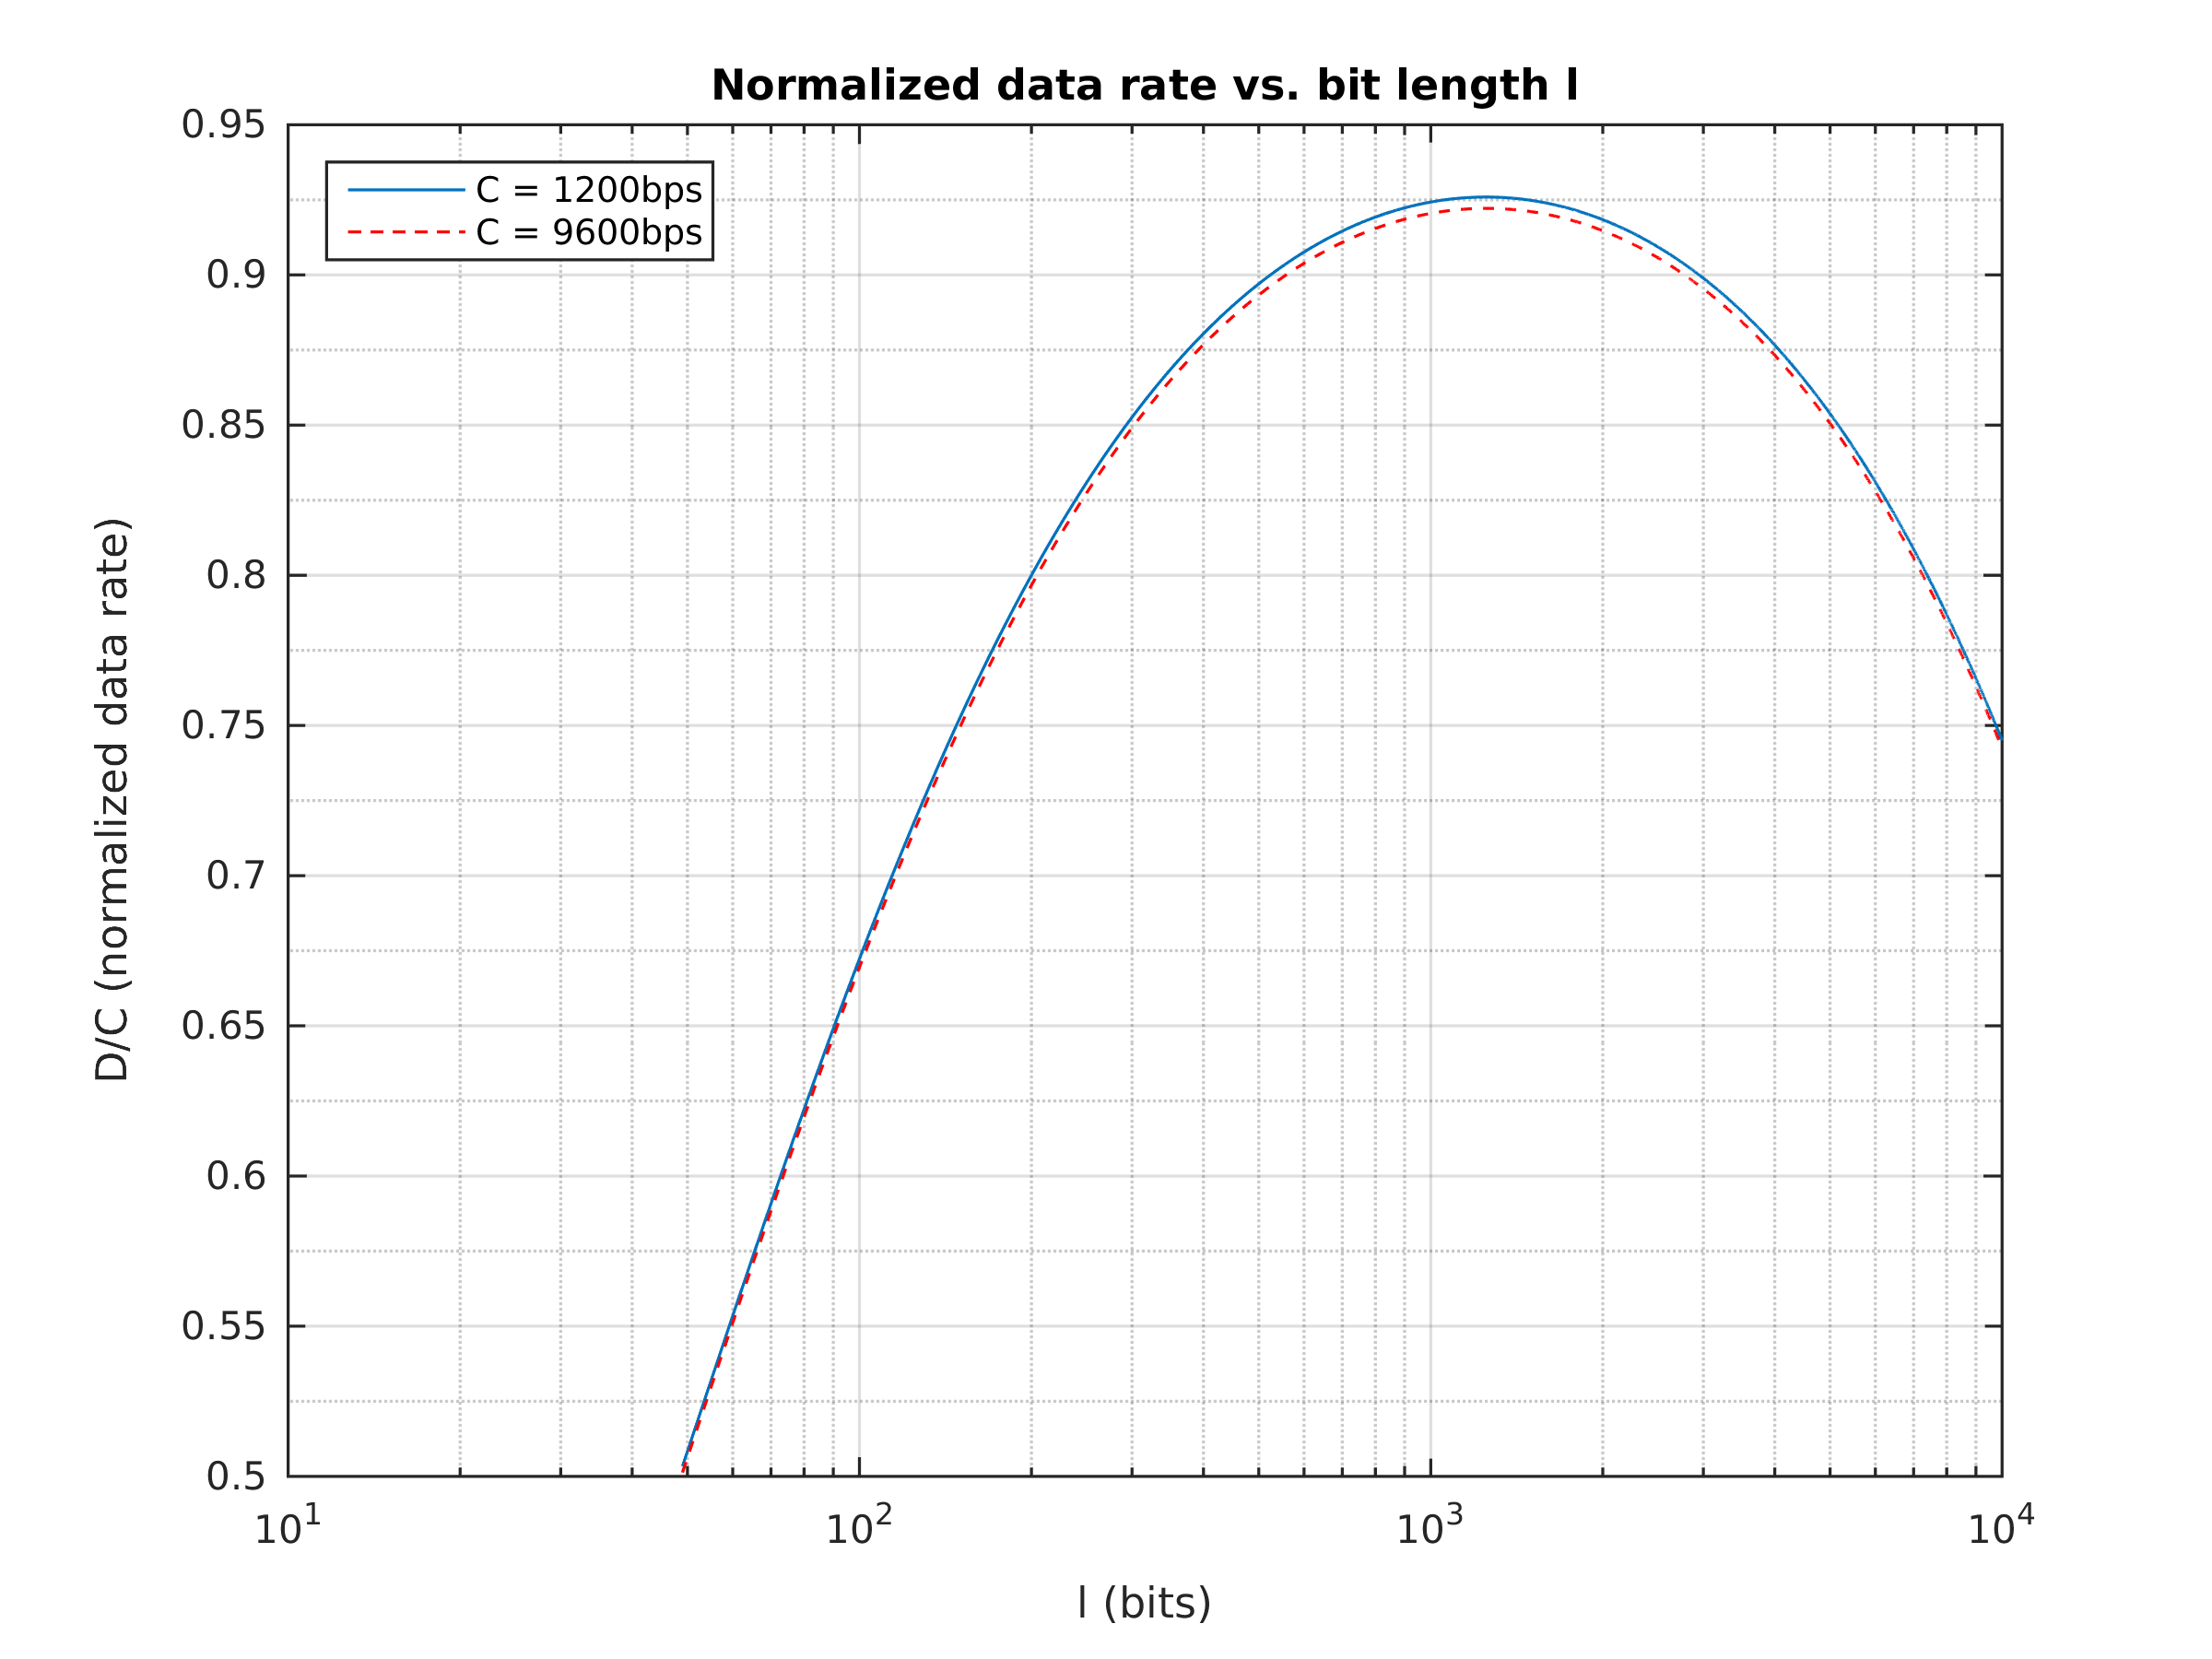
\includegraphics[width=0.6\linewidth]{hw5_1_dr.png}
		\caption{Normalized data throughput rate $D/C$ for go-back-N protocol.}
	\end{figure}
	We can observe that the given these conditions, even with a different link
	speed, the normalized data rate is about the same. This is due to the factor
	$a$ in Eq. (4-10). We know that,
	\begin{equation}
		a = \frac{t_I + t_{out}}{t_I}
	\end{equation}
	Hence, if we change the line speed $C$, $a$ will not vary much since
	$t_{out} \ll t_I$ and $a$ in Equation 1 is dominated by $t_I$.

\section*{Schwartz 4-3}
	\subsection*{Part (a)}
		For this problem, I will use the same method derived in Lecture 21.
		First, let's define:
		\begin{align*}
			t_v &= \text{for a given frame, the time needed for a correct transmission} \\
			N &= \text{total number of retransmission for the frame} \\
			p &= \text{frame error}
		\end{align*}
		From the Law of Total Expectation,
		\begin{align*}
			E[t_v] &= E[E[t_v | N]] \\
			&= E[t_v | N = 0] \cdot P(\left\{ N = 0\right\}) + E[t_v | N = 1] \cdot P(\left\{ N = 1\right\}) + \ldots + E[t_v | N = n] \cdot P(\left\{ N = n\right\}) \\
			&= \sum_{n=0}^{\infty} (t_{\text{ack}} + n \cdot t_{\text{out}} + (n+1) \cdot t_I) p^{n}(1-p) \\
			&= \sum_{n=0}^{\infty} (t_{\text{ack}} + t_I) p^{n}(1-p) + \sum_{n=0}^{\infty} n(t_{\text{out}} + t_I) p^{n}(1-p) \\
			&= (t_{\text{ack}} + t_I) + (1-p)(t_{\text{out}} + t_I)\sum_{n=0}^{\infty} np^{n} \\
			&= \frac{(t_{\text{ack}} + t_I)(1-p) + p(t_{\text{out}} + t_I)}{1-p}
		\end{align*}
		And from this result, we can obtain,
		\begin{align*}
			\lambda_{max} &= \frac{1}{E[t_v]} \\
			&= \frac{1-p}{(t_{\text{ack}} + t_I)(1-p) + p(t_{\text{out}} + t_I)}
		\end{align*}
		After algebraic manipulations on this result, we can obtain,
		\begin{equation}
			\lambda_{max} = \frac{1-p}{t_{T}[1 + (b-1)p]}
		\end{equation}
		\begin{align*}
			\text{where } b = \frac{t_I + t_{\text{out}}}{t_I + t_{\text{ack}}}
		\end{align*}
		%For comparison, plot new lambda_max
	\subsection*{Part (b)}
	%TODO

\section*{Schwartz 4-4}
	\subsection*{Part (a)}
		The protocol will work correctly. With $t_{\text{ack}} > t_{\text{out}}$,
		the sender will continuously send packets without waiting for the timeout
		to finish. However, the receive will eventually ACK the packet.
	\subsection*{Part (b)}
		The timeout function is needed. When sender sends a series of packets to
		the receiver, the packets can be dropped or lost. In this way, there is no
		way for the receiver/sender to react to this situation if no timeout
		function is implemented.
	\subsection*{Part (c)}
		It is guaranteed that the receiver will detect the original (duplicate)
		frame. Since the sequence number of each packet always increments, if the
		receiver receives an identical packet that has a smaller sequence number
		than the current sequence number, the receive will identify this particular
		packet as a duplicate.

\section*{Schwartz 4-7}
	Using Eq. (4-10) in the Schwartz textbook and MATLAB, we can obtain the
	following plot.
	\begin{figure}[!hbt]
		\centering
		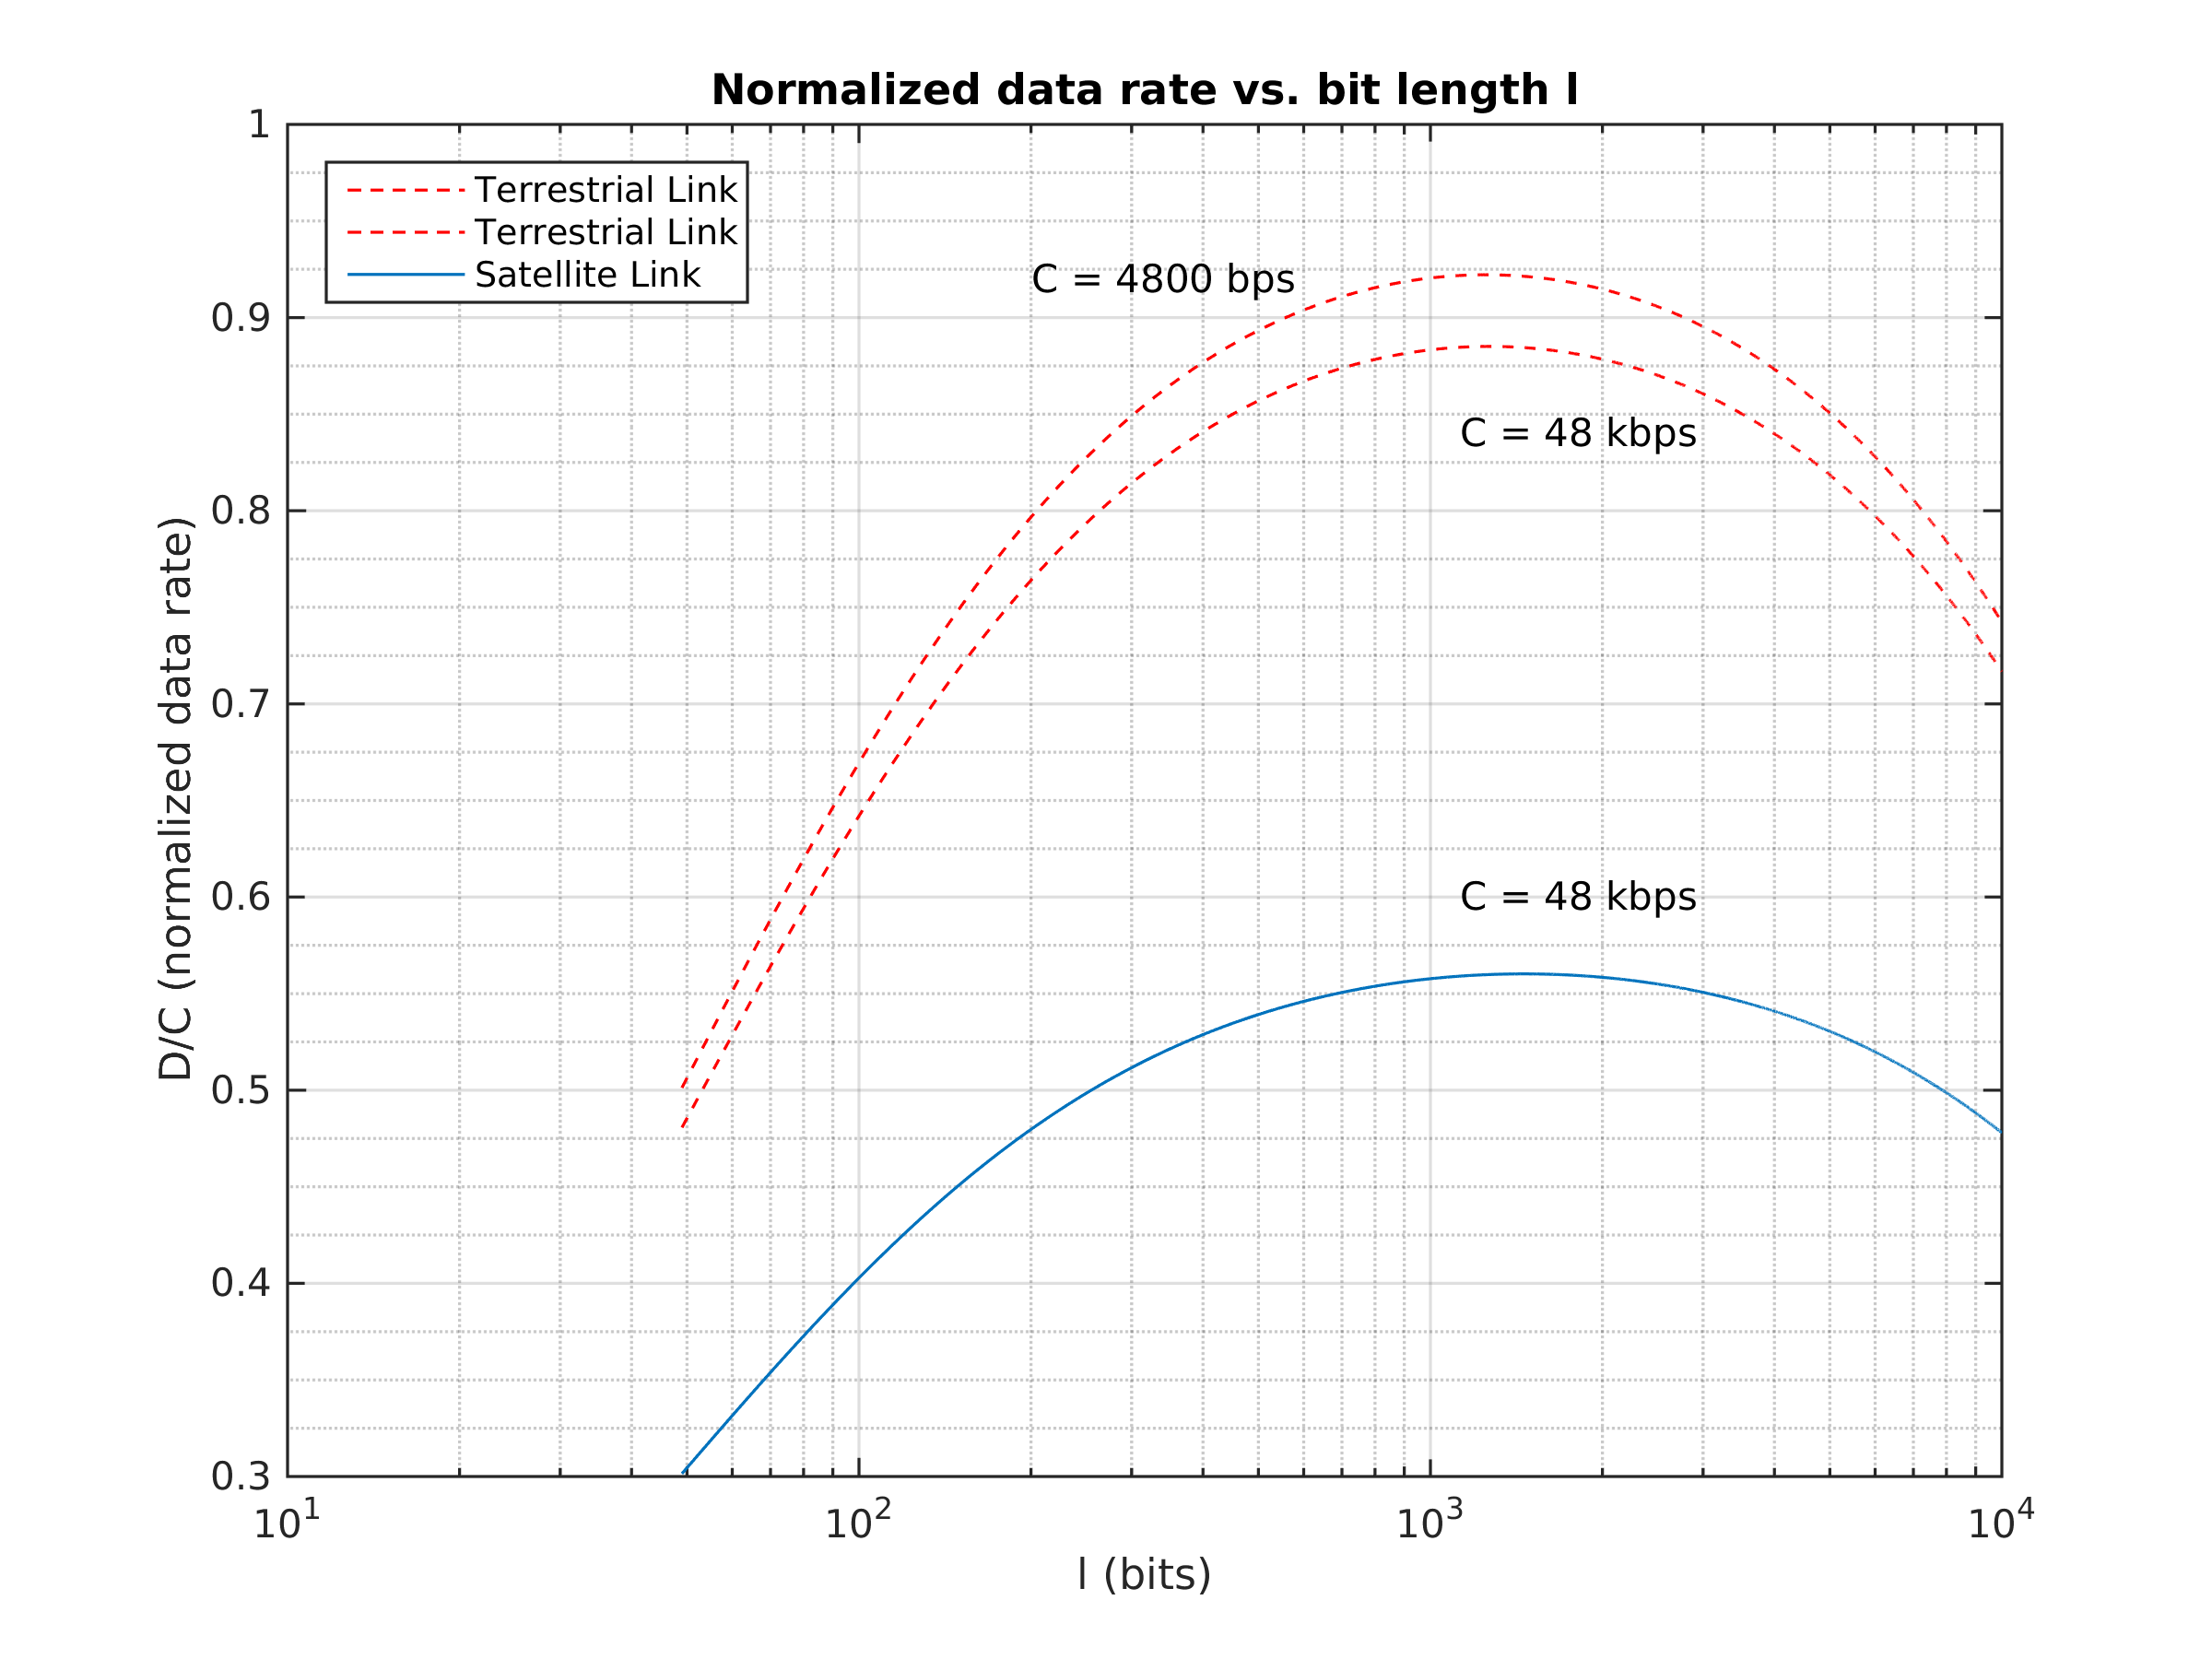
\includegraphics[width=0.6\linewidth]{hw5_3_dr.png}
		\caption{Normalized data throughput rate $D/C$ for terrestrial and satellite link.}
	\end{figure}
	The figure looks identical to Figure 4-8 in Schwartz textbook.

\section*{Schwartz 4-8}
	We need to find the maximum of the normalized rate $D/C$, i.e., $\max\limits_{l}\frac{D}{C}$.
	We can obtain the optimal data length by taking the derviative of $\frac{D}{C}$
	w.r.t. $l$ and set it to 0 to find the corresponding $l$. We know that,
	\begin{align*}
		\frac{D}{C} &= (\frac{l}{l+l'})(\frac{1-p}{1 + (a-1)p}) \\
		&= (\frac{l}{l+l'})(1-p_b)^{l+l'} \text{ for } (a-1)p \ll 1
	\end{align*}
	Hence, by differentiating the above equation w.r.t. $l$ and set the derivative
	to 0, we get,
	\begin{align*}
		l_{\text{opt}} &= \frac{\sqrt{l'} \sqrt{\log{(1-p_{b})}} \sqrt{l\log{(1-p_{b})} - 4} - \sqrt{\log{(1-p_{b})}}}{2 \sqrt{\log{(1-p_{b})}}} \\
		&= \frac{1}{2} \frac{\sqrt{(l')^{2} \log{(1-p_{b})} - 4l'} - \sqrt{\log{(1-p_{b})}}}{\sqrt{\log{(1-p_{b})}}} \\
		&= \frac{l'}{2} ( \sqrt{1 - \frac{4}{l' \log{(1-p_{b})}}} - 1)
	\end{align*}
	We can plug in $l' = 48$ and $p_{b} = 1e-5$ into the equation and we get
	$l_{\text{opt}} \approx 2167$ which matches the general trend in Figure 4-8.

\section*{Schwartz 4-17}

\end{document}
